\section{O avanço tecnológico na sociedade moderna}

A nomenclatura ``era da tecnologia'' ganhou relevância nos últimos anos ao descrever o período contemporâneo em que a humanidade está imersa, onde inúmeras atividades cotidianas são não apenas assistidas, mas, em alguns casos, substancialmente dependentes das maravilhas tecnológicas. Dentro desta linha de pensamento, emerge com notoriedade a importância da Internet, que figura como uma força condutora ao possibilitar avanços notáveis em um lapso temporal reduzido. Concebida pelo cientista britânico \textit{Tim Berners-Lee} em 1989, a Internet remodelou por completo o panorama das comunicações, sendo que, apesar de sua criação relativamente recente, evoluiu para se tornar um epicentro impulsionador de uma metamorfose sem precedentes, ilustrada vividamente na Figura \ref{GlobalInternetUsers}.

\begin{figure}[H]
	\centering
	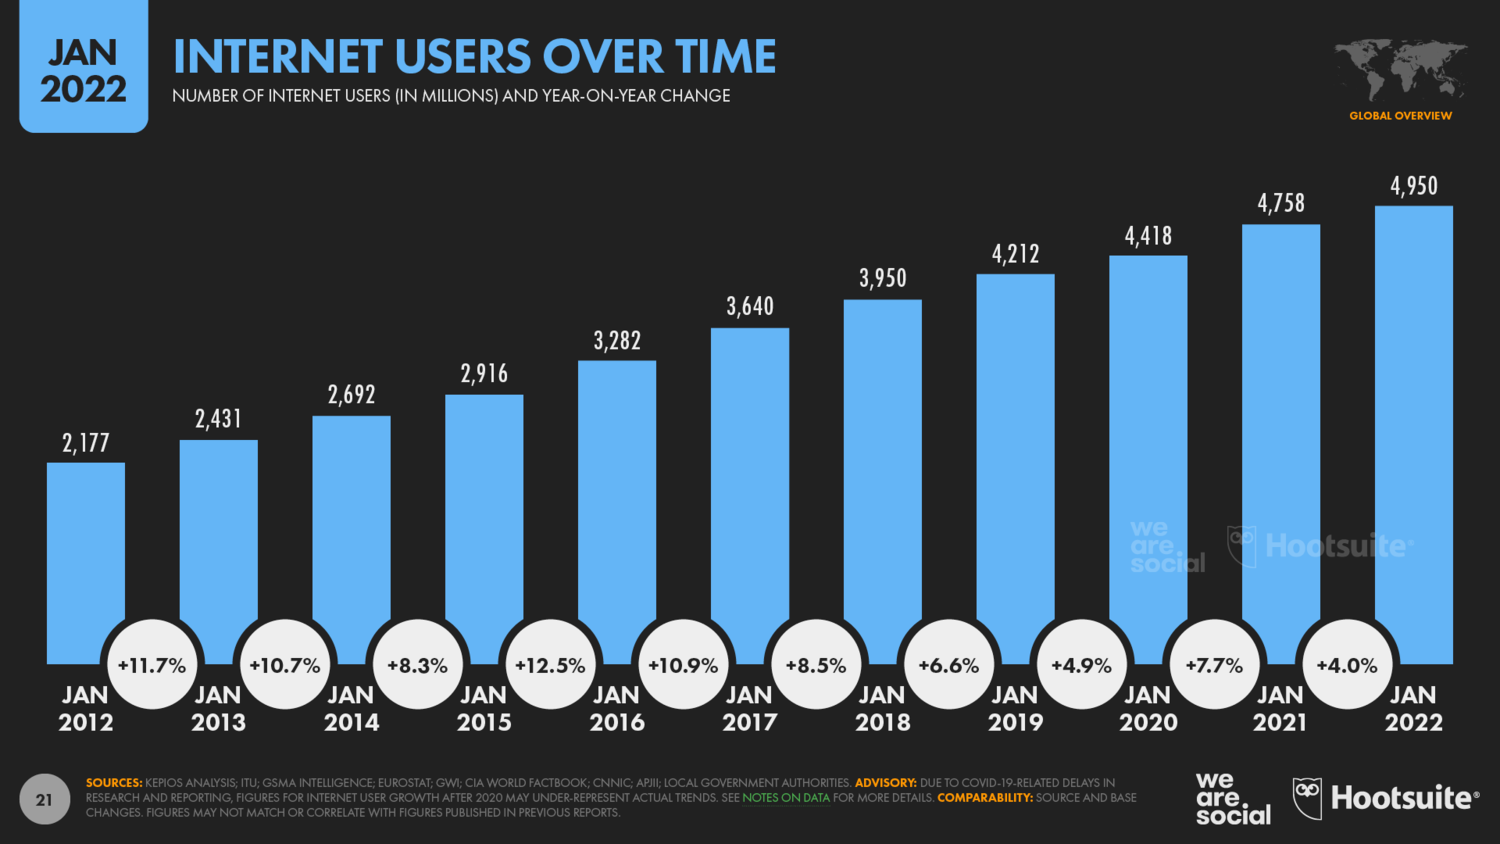
\includegraphics[scale=0.3]{imagens/revisaoLeitura/global_internet_users_over.png}
	\caption{Global Internet Users Over }
	\label{GlobalInternetUsers}
	\fonte{\cite{digital_2022_global_overview_report}}
\end{figure}

Na era tecnológica, a Internet emerge como uma influência transformadora, conectando bilhões de pessoas globalmente e desempenhando um papel central em várias esferas da vida humana. Seu impacto persistirá, moldando o mundo à medida que novas tecnologias e inovações surgem, promovendo um futuro cada vez mais interconectado e globalizado para a humanidade.

